\chapter{VIBEGUARD SYSTEM DESIGN AND ARCHITECTURE}
\label{ch:system_arch}

\section{Conceptual System Architecture}
VibeGuard is architected as an autonomous, edge-resident vibration monitoring and decision-making pipeline. The primary design objective is to perform all sensing, static offset cancellation, feature extraction, temporal persistence filtering, and spectral analysis directly on an embedded microcontroller without relying on remote network connectivity.

Figure~\ref{fig:sys_arch_l1} presents the Level-1 high-level system architecture. The physical system comprises four primary interconnected domains:
\begin{enumerate}
    \item \textbf{Mechanical Testbed:} A guarded 12\,V DC micro metal gear motor coupled to an eccentric mass rotor, anchored to a laminated acrylic baseplate.
    \item \textbf{Sensing Node:} A rigidly clamped Analog Devices ADXL345 triaxial digital accelerometer measuring continuous mechanical acceleration.
    \item \textbf{Embedded Processing Unit:} A 32-bit dual-core 7Semi ESP32-DEVKIT-E microcontroller executing real-time data acquisition, digital signal processing, and state machine transitions.
    \item \textbf{Human-Machine Interface (HMI) and Telemetry:} A common-cathode RGB LED providing instant visual operational status, complemented by structured USB serial telemetry ($115200$\,baud) for validation and historical logging.
\end{enumerate}

\begin{figure}[H]
\centering
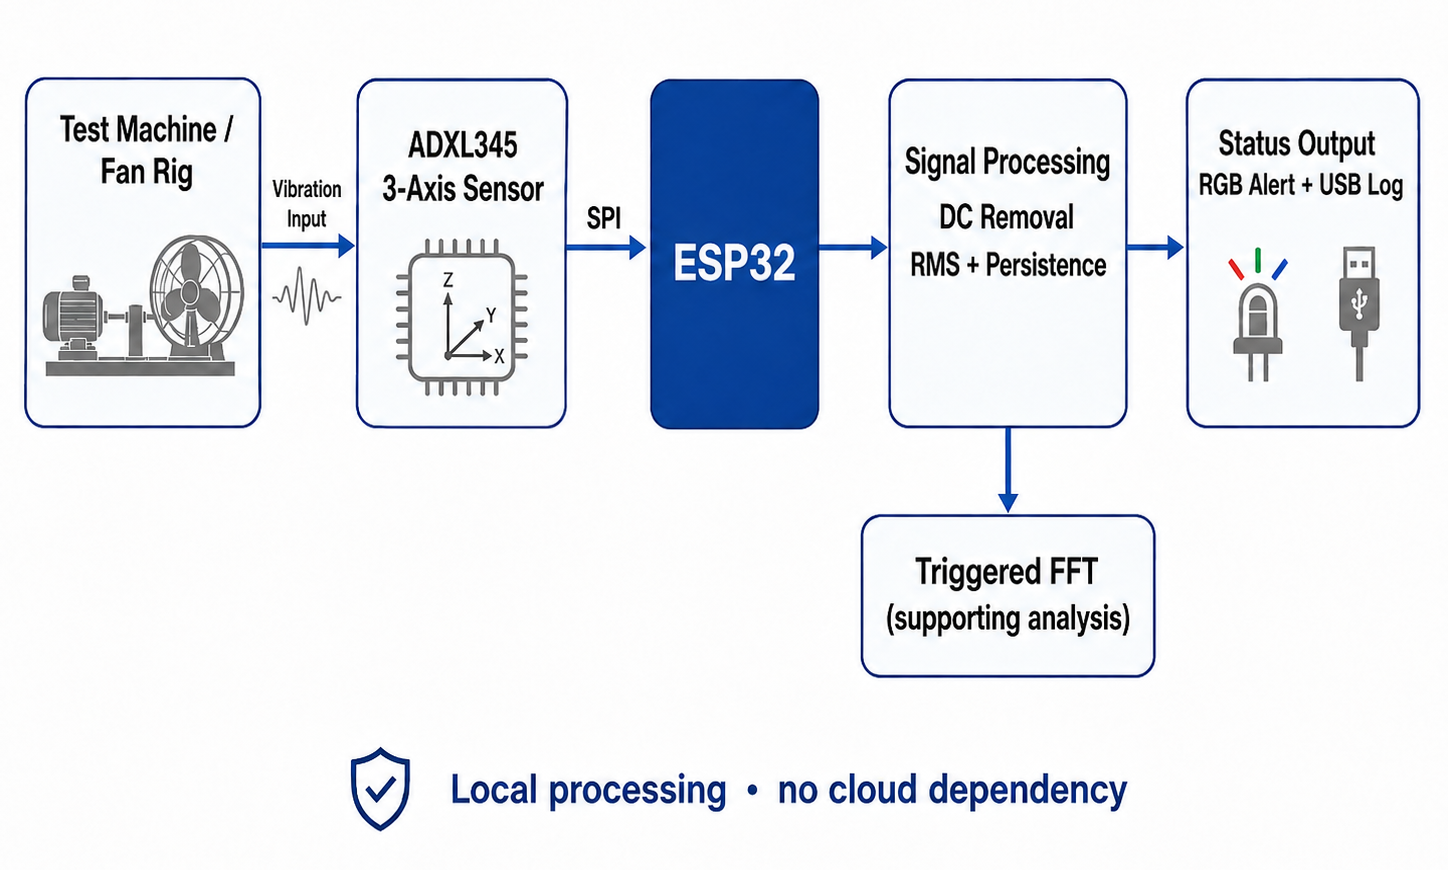
\includegraphics[width=0.88\textwidth]{figures/fig_system_architecture.png}
\caption{VibeGuard Level-1 system architecture block diagram}
\label{fig:sys_arch_l1}
\end{figure}

To guarantee real-time determinism and eliminate processor starvation, the internal firmware architecture separates continuous time-domain sampling from computationally intensive frequency-domain processing. Figure~\ref{fig:dsp_pipeline} details the Level-2 digital signal processing (DSP) and state execution pipeline.

\begin{figure}[H]
\centering
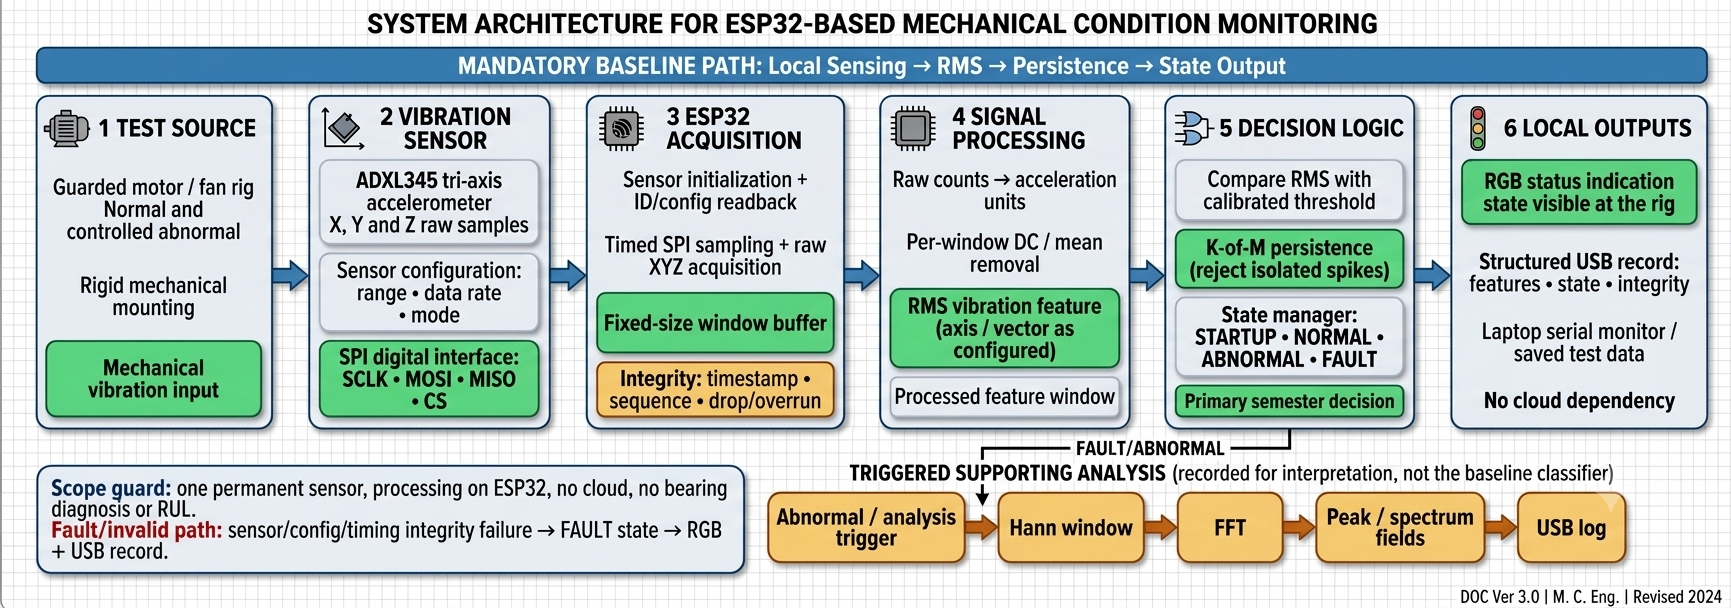
\includegraphics[width=0.92\textwidth]{figures/fig_dsp_pipeline.png}
\caption{VibeGuard Level-2 detailed signal processing and state decision pipeline}
\label{fig:dsp_pipeline}
\end{figure}

\section{Signal Acquisition Flow and Sampling Theory}
\subsection{Sampling Rate and Nyquist Bandwidth Selection}
The rotational speed of the VibeGuard N20 gear motor is nominally 600\,RPM, corresponding to a fundamental mechanical shaft rotational frequency:
\begin{equation}
f_{\mathrm{shaft}} = \frac{600\,\text{RPM}}{60\,\text{s}} = 10.0\,\text{Hz}
\end{equation}
In rotating machinery condition monitoring, diagnosing unbalance, misalignment, and structural resonance requires capturing not only the fundamental rotational frequency ($1X = 10$\,Hz) but also significant higher-order mechanical harmonics ($2X, 3X, \dots, 20X$). 

The ADXL345 digital accelerometer is configured via its internal rate register (\texttt{BW\_RATE}, address \texttt{0x2C}) to an Output Data Rate (ODR) of $f_s = 800$\,Hz. According to the Nyquist-Shannon sampling theorem, the theoretical maximum observable frequency bandwidth without aliasing is:
\begin{equation}
f_{\mathrm{Nyq}} = \frac{f_s}{2} = \frac{800\,\text{Hz}}{2} = 400.0\,\text{Hz}
\end{equation}
A 400\,Hz Nyquist bandwidth encompasses up to the 40th mechanical harmonic ($40X$) of the 10\,Hz shaft frequency. This wide bandwidth guarantees that all significant unbalance harmonics, mechanical rattle, and structural resonance frequencies are captured with high fidelity~\cite{vibeguard_primer2026}.

\subsection{Analysis Window and Spectral Bin Resolution}
Data processing operates over rolling, non-overlapping analysis blocks of $N = 256$ samples per channel. At $f_s = 800$\,Hz, each 256-sample window spans a physical temporal duration of:
\begin{equation}
T_{\mathrm{window}} = \frac{N}{f_s} = \frac{256}{800\,\text{Hz}} = 0.320\,\text{s} = 320\,\text{ms}
\end{equation}
During each 320\,ms window, the rotating shaft completes exactly:
\begin{equation}
N_{\mathrm{cycles}} = T_{\mathrm{window}} \cdot f_{\mathrm{shaft}} = 0.320\,\text{s} \times 10\,\text{Hz} = 3.2\,\text{revolutions}
\end{equation}
Capturing more than 3 complete mechanical cycles per window ensures statistical stability in time-domain RMS calculation. Furthermore, when transformed into the frequency domain via a 256-point FFT, the discrete spectral frequency bin resolution $\Delta f$ is:
\begin{equation}
\Delta f = \frac{f_s}{N} = \frac{800\,\text{Hz}}{256} = 3.125\,\text{Hz / bin}
\end{equation}
With $\Delta f = 3.125$\,Hz, the 10\,Hz fundamental shaft frequency maps cleanly into bin $k = 3$ ($3 \times 3.125 = 9.375$\,Hz) and bin $k = 4$ ($4 \times 3.125 = 12.5$\,Hz), enabling sharp spectral peak detection.

\section{Circuit Schematic and Electrical Power Isolation}
Operating high-current inductive electric motors in close physical proximity to sensitive digital microcontrollers introduces significant risks of electrical noise, ground bounce, and inductive voltage spikes. To guarantee absolute hardware survivability and signal integrity, VibeGuard implements complete electrical power domain isolation.

Figure~\ref{fig:schematic} displays the master circuit schematic of the complete VibeGuard monitoring system.

\begin{figure}[H]
\centering
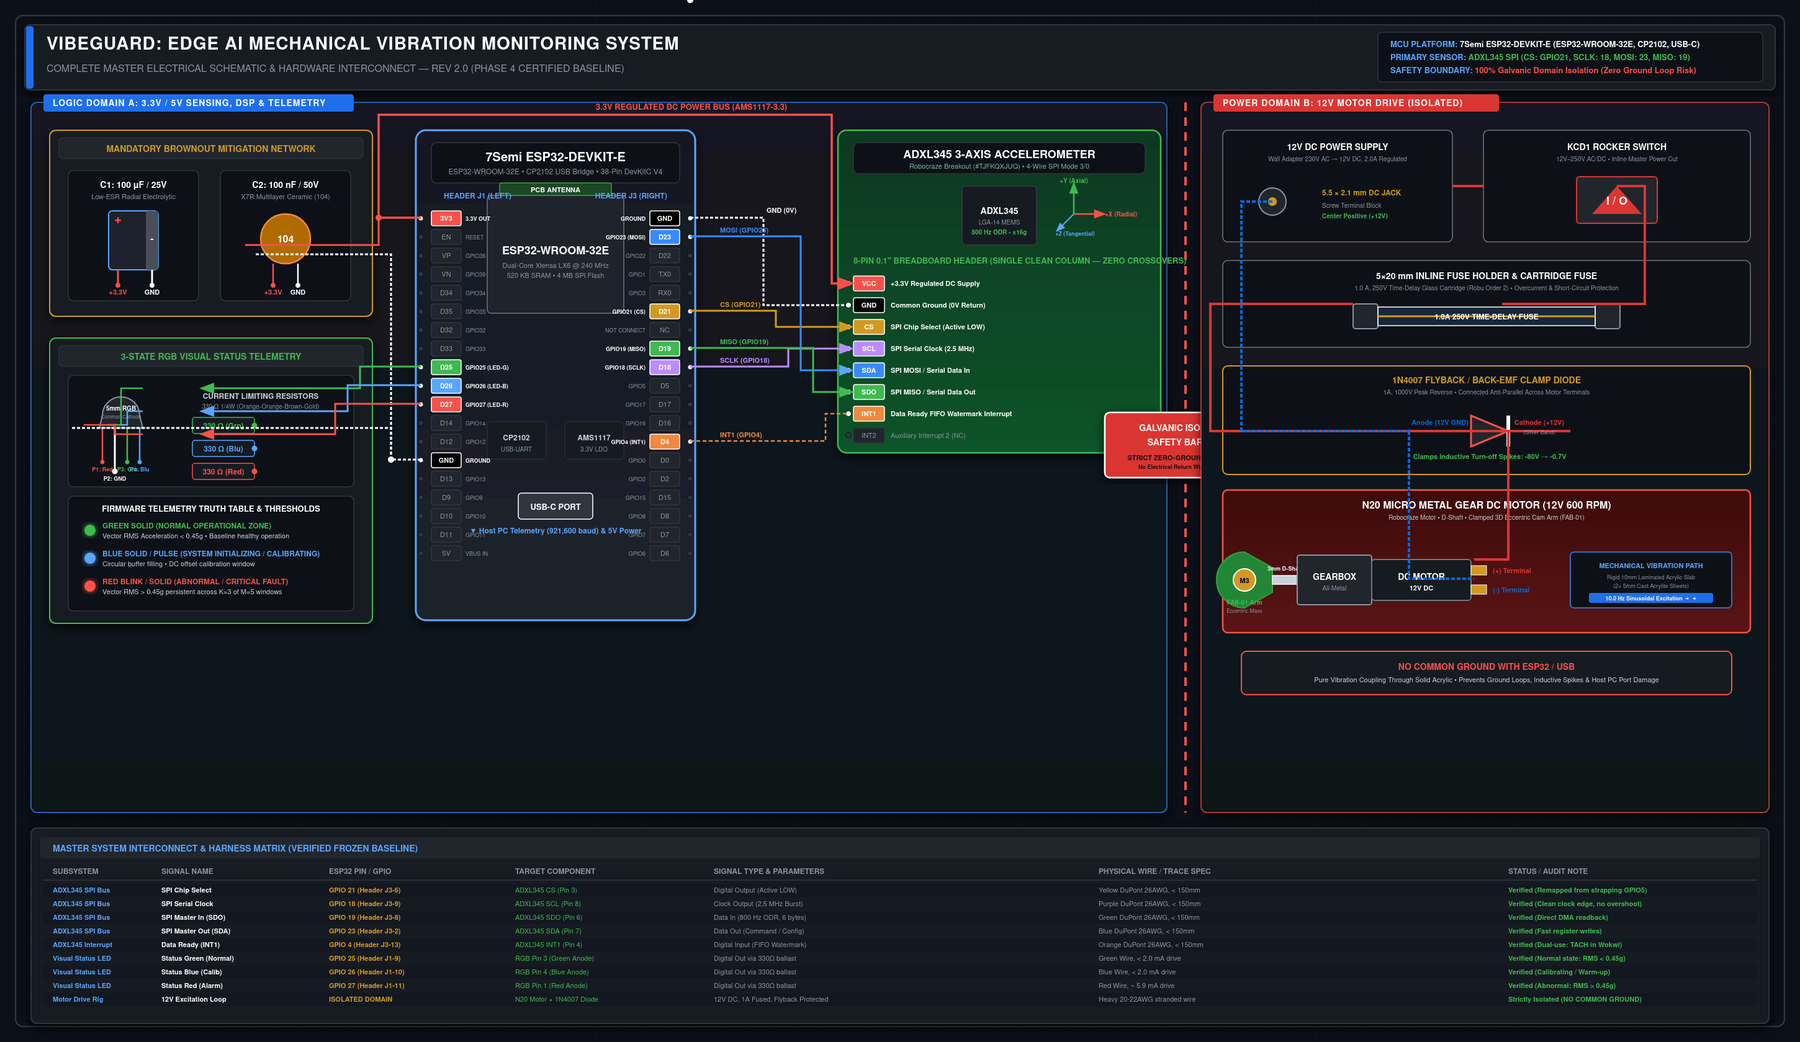
\includegraphics[width=0.92\textwidth]{figures/fig_circuit_schematic.png}
\caption{VibeGuard master electrical circuit schematic}
\label{fig:schematic}
\end{figure}

\subsection{Power Domain Separation and Clamping Circuitry}
The system segregates power into two electrically independent domains:
\begin{enumerate}
    \item \textbf{Logic and Sensing Domain (3.3\,V / 5.0\,V):} The 7Semi ESP32-DEVKIT-E microcontroller is powered via a regulated 5\,V USB connection from the host PC. An onboard AMS1117-3.3 Low-Dropout (LDO) linear voltage regulator steps the 5\,V rail down to a clean 3.3\,V logic rail. The ADXL345 digital accelerometer is powered directly from this 3.3\,V rail, consuming a negligible active current of approximately $140\,\mu\text{A}$.
    \item \textbf{Motor Drive Power Domain (12.0\,V):} The N20 micro metal gear motor is powered by an external 12\,V / 2\,A DC switch-mode power adapter through a heavy-duty $5.5\,\text{mm} \times 2.1\,\text{mm}$ screw-terminal DC barrel jack. Under no circumstances is the 12\,V motor power rail connected to the ESP32 microcontroller or its USB supply.
\end{enumerate}

Figure~\ref{fig:motor_safety} illustrates the dedicated 12\,V motor safety and clamping circuit.

\begin{figure}[H]
\centering
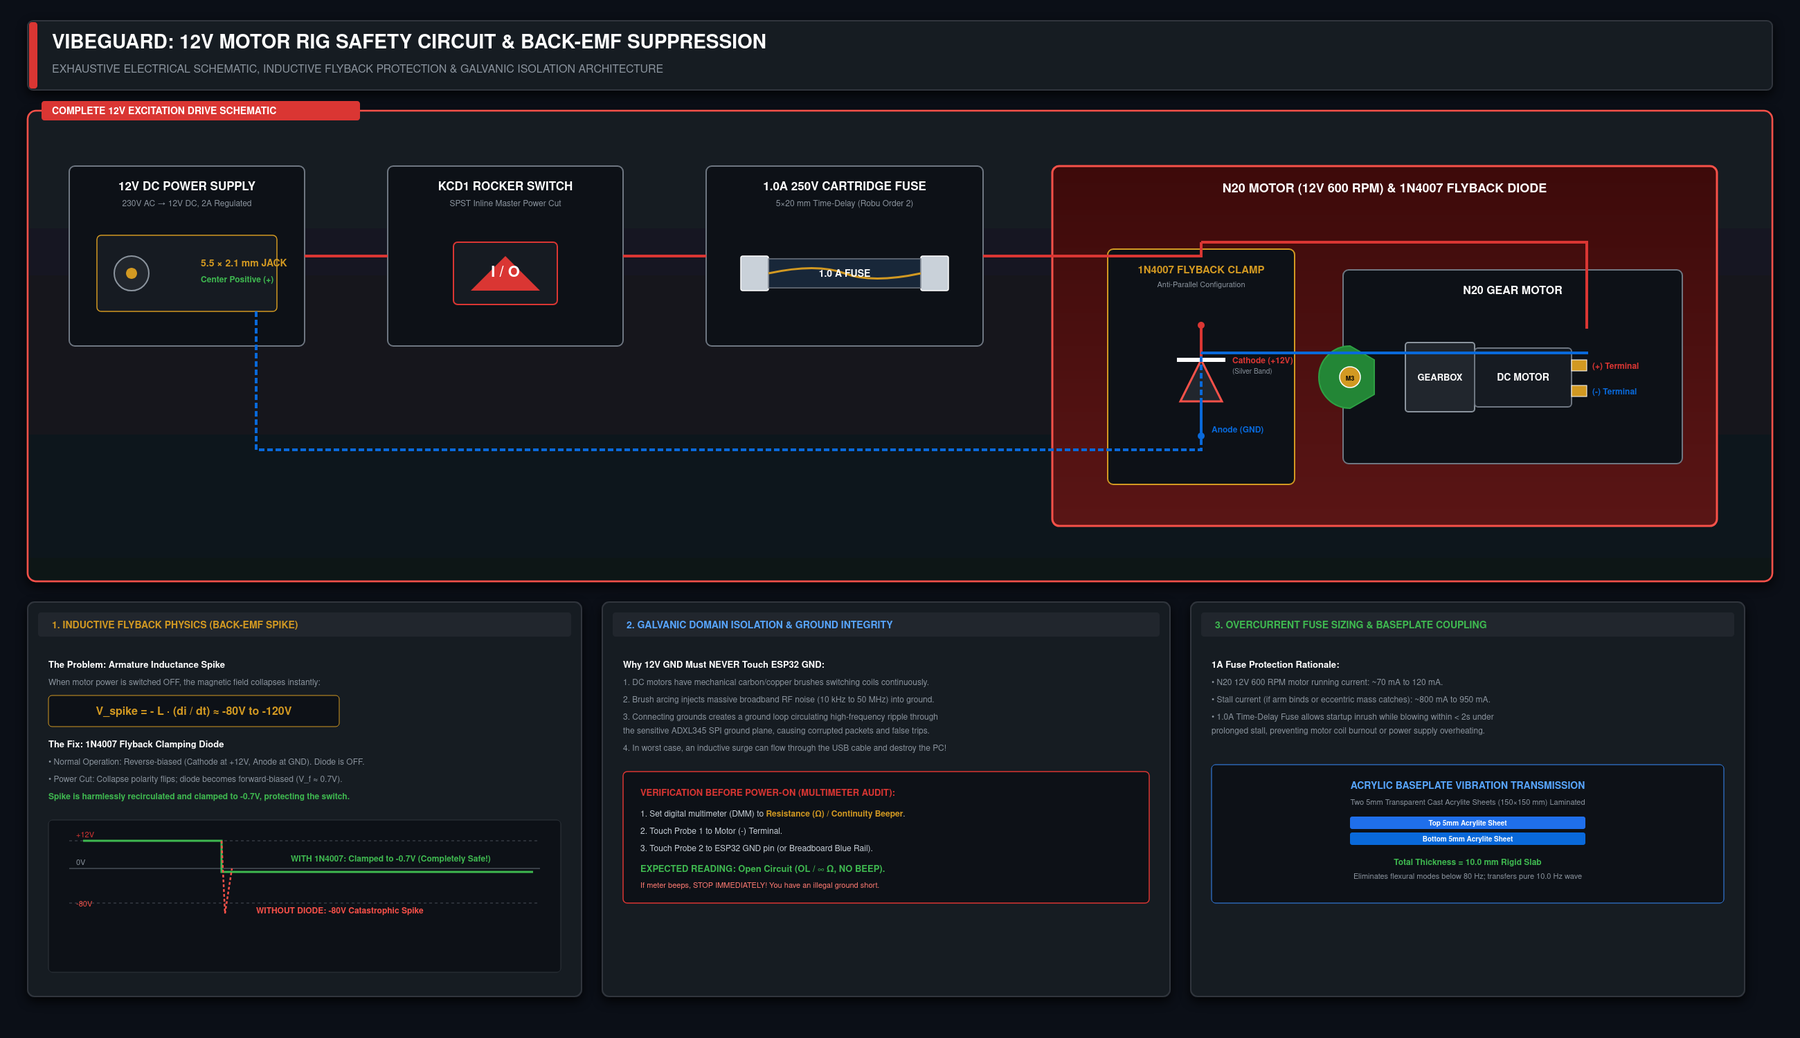
\includegraphics[width=0.75\textwidth]{figures/fig_motor_safety_circuit.png}
\caption{Dedicated 12\,V motor drive safety and inductive clamp circuit}
\label{fig:motor_safety}
\end{figure}

The motor drive loop incorporates three essential protective elements:
\begin{itemize}
    \item \textbf{1A Fast-Acting Cartridge Fuse:} Positioned immediately adjacent to the positive 12\,V input terminal in a $5 \times 20$\,mm screw-cap inline housing, protecting the power supply against mechanical rotor stalls or short circuits.
    \item \textbf{KCD1 Rocker Switch:} A mechanical SPST power disconnect switch providing instant manual emergency shutdown.
    \item \textbf{1N4007 Flyback Suppression Diode:} Connected in reverse-bias across the motor terminals ($V_{\mathrm{RRM}} = 1000$\,V, $I_F = 1$\,A). When power is interrupted, the collapsing magnetic field inside the motor windings induces a high-voltage back-EMF spike ($L \frac{di}{dt} > 100$\,V). The 1N4007 diode clamps this inductive flyback voltage safely to $0.7$\,V, eliminating electrical arcing and ground bounce.
\end{itemize}

\subsection{Brownout Protection and Decoupling Network}
The ESP32 microcontroller contains an integrated internal Brownout Detector (BOD). If the internal 3.3\,V rail sags below the reset threshold of 2.70\,V for more than $2\,\mu\text{s}$, the hardware triggers an immediate brownout reset (\texttt{rst:0x10}). During initialization, internal Wi-Fi calibrations, or high-frequency SPI transfers, current demand can surge transiently to 500\,mA, causing severe voltage drops across long jumper wires.

To eliminate brownout resets, VibeGuard incorporates a dual-capacitor decoupling network connected across the primary 3.3\,V and GND power rails on the breadboard:
\begin{itemize}
    \item \textbf{100\,$\mu$F / 25\,V Electrolytic Bulk Capacitor:} Provides high-energy bulk charge storage to buffer high-current transient spikes.
    \item \textbf{100\,nF (0.1\,$\mu$F) Ceramic Bypass Capacitor:} Features ultra-low Equivalent Series Resistance (ESR) to shunt high-frequency RF switching noise to ground.
\end{itemize}

\section{Sensor Interface and 4-Wire SPI Bus Configuration}
\subsection{SPI Mode and Clocking}
The ADXL345 is configured in 4-wire SPI Mode~3, characterized by:
\begin{itemize}
    \item \textbf{Clock Polarity ($\mathrm{CPOL} = 1$):} SCLK idles HIGH when the bus is inactive.
    \item \textbf{Clock Phase ($\mathrm{CPHA} = 1$):} Data is sampled on the rising (second) clock edge and shifted out on the falling edge.
\end{itemize}
The ESP32 hardware VSPI peripheral is configured to drive SCLK at 5.0\,MHz. Because reading 6 bytes of acceleration data requires transmitting 7 bytes (56 clock cycles), the physical transfer takes:
\begin{equation}
T_{\mathrm{transfer}} = \frac{56\,\text{cycles}}{5 \times 10^6\,\text{Hz}} = 11.2\,\mu\text{s}
\end{equation}
Compared to the 1.25\,ms ($1250\,\mu\text{s}$) sample interval at 800\,Hz ODR, the SPI bus transfer consumes less than 0.9\% of available bus time, leaving over 99\% of CPU time available for signal processing.

\subsection{Strapping Pin Mitigation (GPIO21 Remapping)}
In standard ESP32 DevKit pinout mappings, the default hardware VSPI Chip Select (CS) is tied to GPIO5. However, the ESP32 Silicon Errata and Technical Reference Manual identify GPIO5 as a critical \textbf{boot strapping pin}~\cite{esp32_trm}. During power-on reset, the on-chip ROM bootloader samples GPIO5 to configure internal SDIO timing. If an external peripheral pulls GPIO5 LOW during reset, the bootloader fails to initialize flash memory, resulting in bootloops and serial log corruption.

To permanently eliminate this failure mode, VibeGuard remaps the active-low Chip Select line to \textbf{GPIO21} in firmware. GPIO21 is an unstrapped general-purpose I/O pin, guaranteeing 100\% reliable boot sequences under all power states.

\section{Working Principle and Finite State Machine}
The VibeGuard firmware operates as a deterministic, non-blocking Finite State Machine (FSM). System execution transitions through five distinct operating states, as detailed in Table~\ref{tab:fsm_states} and illustrated in Figure~\ref{fig:dsp_pipeline}.

\begin{table}[H]
\centering
\begin{tabular}{|l|c|l|l|}
\hline
\textbf{Operating State} & \textbf{RGB LED} & \textbf{Condition / Trigger} & \textbf{Firmware Action} \\
\hline
\textbf{STATE\_SELFTEST} & Solid Blue & Hardware Power-on / Reset & Verifies ADXL345 DEVID (0xE5); inits SPI \\
\textbf{STATE\_CALIBRATING} & Flashing Blue & Normal machine run (30\,s) & Computes baseline $\mu_{\mathrm{base}}$ and $\theta_{\mathrm{RMS}}$ threshold \\
\textbf{STATE\_NORMAL} & Solid Green & $a_{\mathrm{vec}} \le \theta_{\mathrm{RMS}}$ & Continuous monitoring; updates rolling RMS \\
\textbf{STATE\_ABNORMAL} & Solid Red & $K \ge 4$ of $M=5$ violations & Asserts alarm; triggers Hann-windowed FFT \\
\textbf{STATE\_FAULT} & Solid White & SPI disconnect / FIFO overflow & Halts processing; flags telemetry invalid \\
\hline
\end{tabular}
\caption{VibeGuard Finite State Machine (FSM) state definitions}
\label{tab:fsm_states}
\end{table}

\subsection{State Transition Logic}
\begin{enumerate}
    \item \textbf{Self-Test State:} Upon power-on, the ESP32 initializes the serial console and configures the VSPI bus. It reads the \texttt{DEVID} register (address \texttt{0x00}) of the ADXL345. If the returned byte does not match the factory hardcoded value of \texttt{0xE5}, the system immediately enters \texttt{STATE\_FAULT} (White LED). If valid, it configures registers and enters \texttt{STATE\_CALIBRATING}.
    \item \textbf{Calibrating State:} The system samples 100 consecutive baseline windows (32\,seconds) while the machine runs under known normal conditions. It computes the long-term baseline mean vector RMS ($\mu_{\mathrm{base}}$) and standard deviation ($\sigma_{\mathrm{base}}$). The anomalous vibration threshold $\theta_{\mathrm{RMS}}$ is established via statistical margin:
    \begin{equation}
    \theta_{\mathrm{RMS}} = \mu_{\mathrm{base}} + 3.5 \cdot \sigma_{\mathrm{base}}
    \label{eq:threshold}
    \end{equation}
    Once calibration completes, the threshold is permanently frozen, and the system transitions to \texttt{STATE\_NORMAL} (Green LED).
    \item \textbf{Normal Monitoring State:} In this state, the MCU acquires continuous 256-sample windows, computes zero-mean DC cancellation, and calculates the triaxial Vector RMS $a_{\mathrm{vec}}$. If $a_{\mathrm{vec}} \le \theta_{\mathrm{RMS}}$, the Green LED remains lit.
    \item \textbf{Abnormal State \& Persistence Logic:} If an individual window exceeds the threshold ($a_{\mathrm{vec}} > \theta_{\mathrm{RMS}}$), an anomaly flag is queued into a 5-window circular history buffer ($M = 5$). If at least $K = 4$ out of the last $M = 5$ windows violate the threshold, the system transitions to \texttt{STATE\_ABNORMAL} (Red LED). This persistence filter rejects transient mechanical jolts (e.g., accidental table bumps). Simultaneously, the firmware triggers a 256-point Hann-windowed FFT to isolate dominant harmonic peak frequencies.
    \item \textbf{Fault / Invalid State:} If sensor communication fails, bus readback returns static zeros, or FIFO buffer overrun occurs, the system asserts \texttt{STATE\_FAULT}. This guarantees that sensor disconnects are never falsely interpreted as normal machine health.
\end{enumerate}

\section{Human-Machine Interface and Telemetry Protocol}
VibeGuard provides dual-tier state visualization:
\begin{itemize}
    \item \textbf{Local Optical HMI:} A high-brightness common-cathode RGB LED provides instantaneous, non-verbal machine condition status to floor operators. Connected via 330\,$\Omega$ current-limiting resistors, the channels map to Green (GPIO25), Blue (GPIO26), and Red (GPIO27).
    \item \textbf{Structured USB Serial Telemetry:} The onboard Silicon Labs CP2102 USB-to-UART bridge streams comma-separated ASCII telemetry packets at $115200$\,baud at 3.125\,Hz (one record per 320\,ms window). The standardized record format is structured as follows:
    \begin{center}
    \texttt{\$VBD,seq,timestamp\_ms,rms\_x,rms\_y,rms\_z,rms\_vec,state,f\_peak1,a\_peak1*CS}
    \end{center}
    This standardized NMEA-style telemetry format provides complete traceability, allowing host-side software to parse, archive, and verify all raw calculations.
\end{itemize}

\section{Summary}
This chapter detailed the comprehensive system design and architecture of VibeGuard. The Level-1 and Level-2 architectures showed how real-time acquisition is decoupled from on-demand spectral processing. Sampling at 800\,Hz provides a 400\,Hz Nyquist bandwidth and 3.125\,Hz spectral bin resolution across 256-sample windows. The electrical design guarantees complete power domain isolation between the 12\,V inductive motor circuit and the 3.3\,V/5.0\,V digital logic, protected by a 1A fuse, 1N4007 flyback diode, and a dual-capacitor brownout decoupling network. Finally, remapping Chip Select to GPIO21 eliminated ESP32 strapping pin boot conflicts, and the 5-state FSM ensured deterministic operation and transient noise rejection.
